 \section{Cable}
 
 It exist a certain number of different method to simulate a cable from finite elements to lumped mass
 with different implementations in each cases.
 
\subsubsection*{The simplest model}

If the cable is taken as a simple pendulum (lumped mass) of mass $m$ and length $l$ when the towed is at a constant speed 
and constant heading, the equilibrium state is researched.


\begin{figure}[H]
\centering
\psscalebox{0.8 0.8} % Change this value to rescale the drawing.
{
% \usepackage[usenames,dvipsnames]{pstricks}
% \usepackage{epsfig}
% \usepackage{pst-grad} % For gradients
% \usepackage{pst-plot} % For axes
% \usepackage[space]{grffile} % For spaces in paths
% \usepackage{etoolbox} % For spaces in paths
% \makeatletter % For spaces in paths
% \patchcmd\Gread@eps{\@inputcheck#1 }{\@inputcheck"#1"\relax}{}{}
% \makeatother
% % User Packages:
% \usepackage{amsmath}
% \usepackage{amsfonts}
% \usepackage{amssymb}
% \usepackage{algorithm}
% \usepackage{algorithmic}
% 
\psscalebox{1.0 1.0} % Change this value to rescale the drawing.
{
\begin{pspicture}(0,-2.5449028)(7.8730617,2.5449028)
\definecolor{colour0}{rgb}{0.015686275,0.17254902,0.6666667}
\definecolor{colour1}{rgb}{0.19215687,0.80784315,0.07058824}
\psline[linecolor=black, linewidth=0.04](3.9089148,1.8969576)(5.087519,1.8969576)
\psline[linecolor=black, linewidth=0.04](4.3086305,1.8825132)(2.4941862,-0.9530424)
\psline[linecolor=black, linewidth=0.02, arrowsize=0.05291667cm 2.0,arrowlength=1.4,arrowinset=0.0]{->}(2.4910214,-0.9562069)(2.1720343,-1.4675993)
\psline[linecolor=black, linewidth=0.02, arrowsize=0.05291667cm 2.0,arrowlength=1.4,arrowinset=0.0]{->}(2.5062113,-0.9815234)(3.0176039,-1.3106374)
\psline[linecolor=red, linewidth=0.03, arrowsize=0.05291667cm 2.0,arrowlength=1.4,arrowinset=0.0]{->}(2.4634843,-0.9416389)(0.6248878,-0.9416389)
\psline[linecolor=black, linewidth=0.03, arrowsize=0.05291667cm 2.0,arrowlength=1.4,arrowinset=0.0]{->}(2.4712036,-0.94421196)(2.4712036,-2.5091243)
\psline[linecolor=colour0, linewidth=0.03, arrowsize=0.05291667cm 2.0,arrowlength=1.4,arrowinset=0.0]{->}(2.4749463,-0.9205862)(2.4819639,0.6092383)
\psarc[linecolor=black, linewidth=0.03, linestyle=dashed, dash=0.17638889cm 0.10583334cm, dimen=outer, showpoints=true, arrowsize=0.05291667cm 2.0,arrowlength=1.4,arrowinset=0.0]{<-}(4.3055897,1.8829225){0.5368421}{239.0}{360.0}
\pscircle[linecolor=colour1, linewidth=0.04, fillstyle=solid,fillcolor=colour1, dimen=outer](2.4808948,-0.9663335){0.14177215}
\rput[bl](5.136343,1.3518596){$\theta$}
\rput[bl](2.9794803,-1.2677482){$\vec{u_{\theta}}$}
\rput[bl](1.7402645,-1.4873561){$\vec{u_{r}}$}
\rput[bl](0.0,-0.8332749){$\vec{F_{fluid}}$}
\rput[bl](2.0186048,0.35742274){$\vec{\Pi}$}
\rput[bl](2.5953488,-2.5449028){$\vec{w}$}
\psline[linecolor=black, linewidth=0.012](4.3382597,2.3725133)(4.142704,1.9058465)
\psline[linecolor=black, linewidth=0.012](4.1752973,2.3725133)(3.9797416,1.9058466)
\psline[linecolor=black, linewidth=0.012](4.990112,2.3725133)(4.794556,1.9058466)
\psline[linecolor=black, linewidth=0.012](4.8271494,2.3725133)(4.6315937,1.9058466)
\psline[linecolor=black, linewidth=0.012](4.664186,2.3725133)(4.4686303,1.9058466)
\psline[linecolor=black, linewidth=0.012](4.501223,2.372513)(4.3056674,1.9058465)
\psline[linecolor=black, linewidth=0.012](5.1530747,2.372513)(4.9575195,1.9058465)
\rput[bl](3.2064939,-0.22996545){$(m,l)$}
\psline[linecolor=black, linewidth=0.04, arrowsize=0.05291667cm 2.0,arrowlength=1.4,arrowinset=0.0]{->}(5.5277476,2.0859988)(7.966104,2.0859988)
\rput[bl](6.5798025,2.2449028){$\vec{v_c}$}
\end{pspicture}
}


}
\caption{Representation of cable as a simple pendulum}
\label{fig:model_pendulum}
\end{figure}


$\vec{w}$ is the gravitational force and $\vec{\Pi}$ represent the Archimedes principle, $\vec{F_{fluid}}$ is the resistance due to the fluid and $\vec{T}$ is the force of the base on the cable. $\vec{v_c}$ is the speed of the base (e.g.\ the boat) and $(m,l)$ is the mass and length of the pendulum. If the system is at equilibrium then the speed of the cable is the same as the speed of the base. 

%\begin{align}
\begin{equation}
 \vec{0} = \vec{T}+\vec{F_{fluide}}+\vec{w}+\vec{\Pi}\\
 \label{equ_Stab_1}
\end{equation}


Where if $C_D$ is the drag coefficient $\rho$ is the fluid density, $r$ is the radius of the cable:


{
\begin{align}
\centering
\vec{F_{fluide}} &= -C_D (2 r l) \rho \frac{ \|v_c\|}{2} \cdot \vec{v_c} \\
\vec{w} &= m \cdot \vec{g} \\
\vec{\Pi} &= - \rho \pi r^2 l \cdot \vec{g}
\end{align}
}
If~\ref{equ_Stab_1} is projected on $\vec{u_{\theta}}$ to get rid off the unknown force $\vec{T}$ the result is:

\begin{equation}
 0 = (m g - l \rho \pi r^2 g) \cdot \sin(\theta)-C_D l 2 r \rho \frac{v_c^2}{2} \cdot \cos(\theta)\\
 \label{equ_Stab_2}
\end{equation}

Thus the angle $\theta$ can be found if the cable is more heavy enough ($m -l \rho \pi r^2 > 0)$ i.e.\ the cable is more dense than the fluid otherwise the cable should be always on the surface:

\begin{equation}
 \theta = \arctan(\frac{C_D l 2 r \rho}{2 g \cdot (m - l \rho \pi r^2)} \cdot v_c^2)\\
 \label{equ_theta_1}
 \end{equation}
 
With this formula the depth of the end of the pendulum can be computed with different parameters, linear mass of the cable \ref{fig:depth_mass_speed_pendulum}  or the length of the cable depending 
 
 \begin{figure}[H]
\centering
    \begin{minipage}[b]{0.4\textwidth}
    \centering
    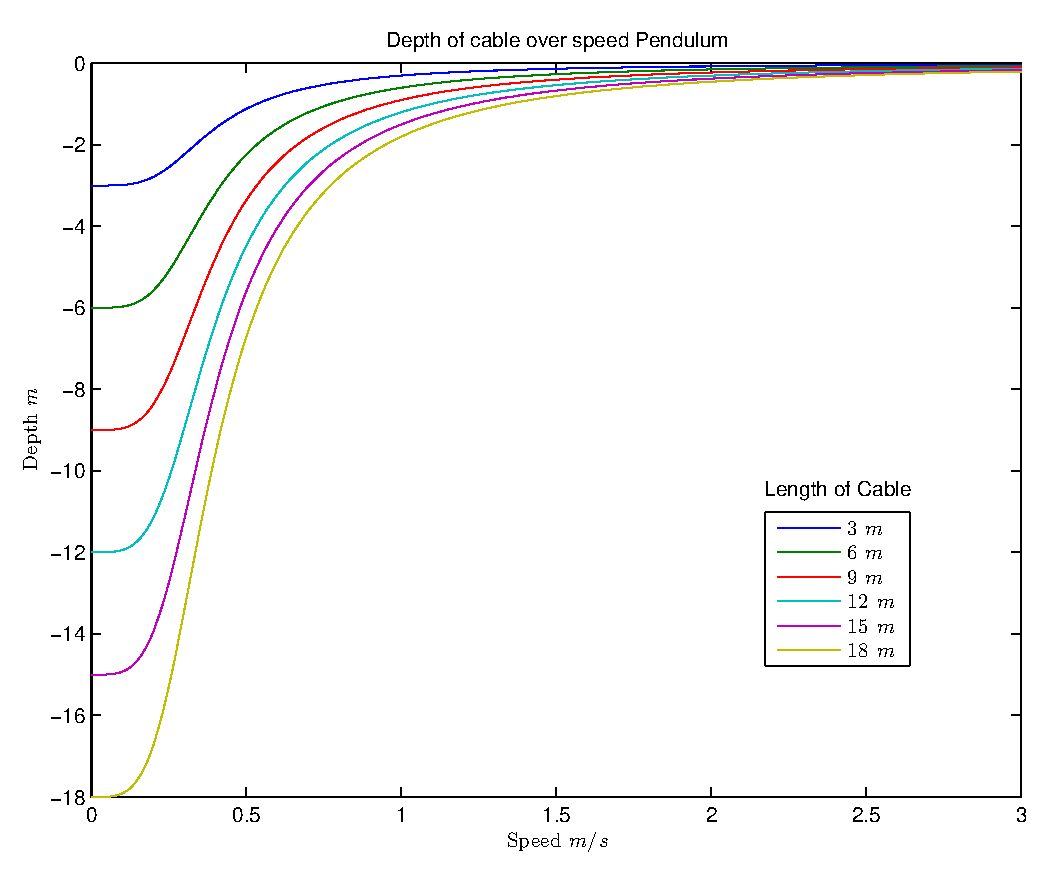
\includegraphics[scale=0.4,angle=0]{depth_length_speed_pendulum}
    \caption{Profile of Depth over Speed of base depending on length of the cable.}
    \label{fig:depth_mass_speed_pendulum}
    \end{minipage}
    \hfill
    \begin{minipage}[b]{0.4\textwidth}
    \centering
    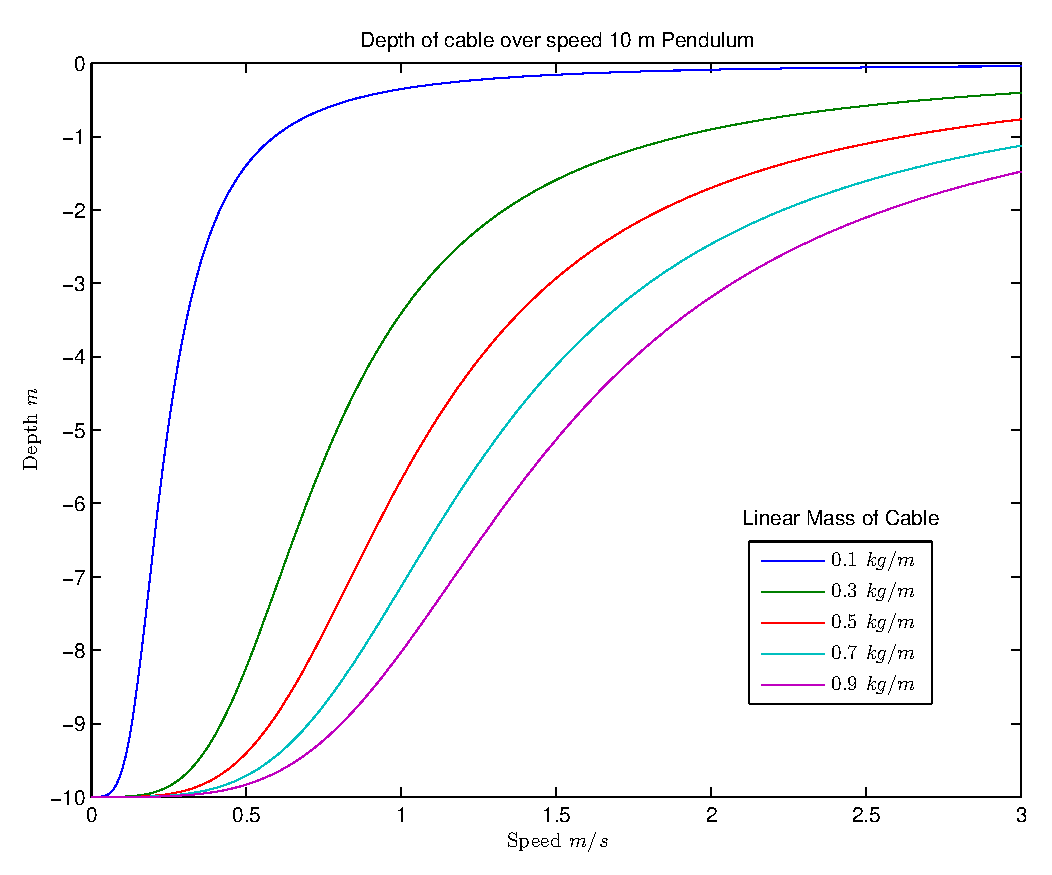
\includegraphics[scale=0.4,angle=0]{depth_mass_speed_pendulum}
    \caption{Profile of Depth over Speed of base depending on linear mass of the cable.}
    \label{fig:depth_length_speed_pendulum}
    \end{minipage}
\end{figure}

\subsubsection*{Finite Elements Method}
 
 
 This method discretize the cable to small elements in the following drawing $T$ represent the tension from the other elements of the cable, $W$ the weight of the cable, $F_N$ and: $F_T$ represent the hydrodynamics forces:
 
\begin{figure}[H]
\centering
\psscalebox{0.40 0.40} % Change this value to rescale the drawing.
{
% \usepackage[usenames,dvipsnames]{pstricks}
% \usepackage{epsfig}
% \usepackage{pst-grad} % For gradients
% \usepackage{pst-plot} % For axes
% \usepackage[space]{grffile} % For spaces in paths
% \usepackage{etoolbox} % For spaces in paths
% \makeatletter % For spaces in paths
% \patchcmd\Gread@eps{\@inputcheck#1 }{\@inputcheck"#1"\relax}{}{}
% \makeatother
% % User Packages:
% \usepackage{amsmath}
% \usepackage{amsfonts}
% \usepackage{amssymb}
% \usepackage{algorithm}
% \usepackage{algorithmic}
% 
\psscalebox{1.0 1.0} % Change this value to rescale the drawing.
{
\begin{pspicture}(0,-3.0463762)(11.863704,3.0463762)
\definecolor{colour0}{rgb}{0.6117647,0.6117647,0.6117647}
\psellipse[linecolor=black, linewidth=0.04, dimen=outer](2.9514816,-1.3041397)(0.89,1.55)
\psbezier[linecolor=black, linewidth=0.04](2.610053,0.1315745)(3.1814816,0.48871735)(8.281482,3.0887175)(9.038625,3.017288785661975)
\psbezier[linecolor=black, linewidth=0.04](9.022083,2.99774)(9.422083,2.3691685)(9.710053,1.6097699)(9.638624,0.13834141724091809)
\psbezier[linecolor=black, linewidth=0.04](3.210053,-2.7421098)(3.7814817,-2.3849669)(8.881481,0.21503314)(9.638624,0.14360457513566247)
\psline[linecolor=black, linewidth=0.04, arrowsize=0.05291667cm 2.0,arrowlength=1.4,arrowinset=0.0]{->}(3.0074077,-1.1985842)(0.77037054,-2.5615473)
\psline[linecolor=black, linewidth=0.04, arrowsize=0.05291667cm 2.0,arrowlength=1.4,arrowinset=0.0]{->}(9.511111,1.8680824)(11.496297,2.5643787)
\psline[linecolor=black, linewidth=0.04, arrowsize=0.05291667cm 2.0,arrowlength=1.4,arrowinset=0.0]{<->}(4.5185184,2.4903047)(5.0962963,1.4532676)(6.711111,2.2828972)
\psline[linecolor=black, linewidth=0.04, arrowsize=0.05291667cm 2.0,arrowlength=1.4,arrowinset=0.0]{->}(5.4074078,0.40141577)(5.392593,-3.139325)
\rput[bl](10.503704,1.1569713){$T(l+dl)$}
\rput[bl](1.762963,-2.8726583){$T(l)$}
\rput[bl](5.9111114,-2.3985841){W}
\rput[bl](3.6740742,2.6680825){$F_N(l)$}
\rput[bl](6.711111,2.534749){$F_T(l)$}
\psline[linecolor=colour0, linewidth=0.03, linestyle=dashed, dash=0.17638889cm 0.10583334cm](2.9925928,-1.1985842)(0.0,-1.1985842)
\psarc[linecolor=black, linewidth=0.04, dimen=outer, showpoints=true, arrowsize=0.05291667cm 2.0,arrowlength=1.4,arrowinset=0.0]{->}(2.9925928,-1.2011385){0.6722861}{180.0}{210.0}
\rput[bl](1.4125161,-0.63459957){$\theta(l)$}
\end{pspicture}
}


}
    \caption{Representation of a finite elements (see~\cite{obligado2013experimental}).}
    \label{fig:finite_elem}
\end{figure}

In general this method is heavy on computational resources due to matrix inversion at each step to compute the solution.
 
 
\subsubsection*{Lumped mass}
 
The cabled is divided in in a certain number of and each segment can be viewed as a mass damped spring system, 
the spring is to simulate elongation of the cable in some cases:

\begin{figure}[H]
\centering
    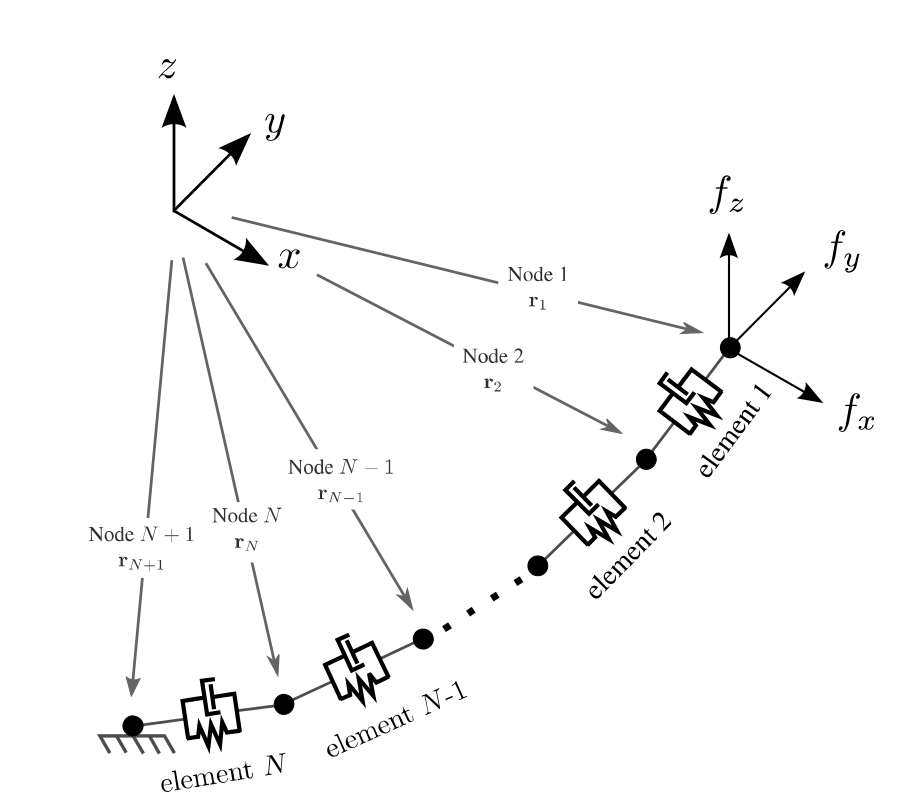
\includegraphics[scale=0.15,angle=0]{damped_spring_lm.png}
    \caption{Representation of Lumped Mass model (see~\cite{masciola2014extending}).}
    \label{fig:lm_damped}
\end{figure}

This model is in general faster to execute because of it does note need the computing of a matrix inverse.
 
\section{Sailboat model}

The model of the sailboat come from~\cite{Melin2016} a modified version of the model in~\cite{LeBars2013}.



\begin{figure}[H]
\centering
\psscalebox{0.45 0.45} % Change this value to rescale the drawing.
{
% \usepackage[usenames,dvipsnames]{pstricks}
% \usepackage{epsfig}
% \usepackage{pst-grad} % For gradients
% \usepackage{pst-plot} % For axes
% \usepackage[space]{grffile} % For spaces in paths
% \usepackage{etoolbox} % For spaces in paths
% \makeatletter % For spaces in paths
% \patchcmd\Gread@eps{\@inputcheck#1 }{\@inputcheck"#1"\relax}{}{}
% \makeatother
% % User Packages:
% \usepackage{amsmath}
% \usepackage{amsfonts}
% \usepackage{amssymb}
% \usepackage{algorithm}
% \usepackage{algorithmic}
\psscalebox{1.0 1.0} % Change this value to rescale the drawing.
{
\begin{pspicture}(0,-6.3229065)(27.976694,6.3229065)
\definecolor{colour6}{rgb}{0.627451,0.627451,0.627451}
\definecolor{colour7}{rgb}{0.40392157,0.3882353,0.3882353}
\pspolygon[linecolor=black, linewidth=0.04, fillstyle=solid,fillcolor=black](4.2265778,0.6801973)(4.2265778,0.6687973)(4.1737776,0.6687973)(4.1737776,0.6801973)
\pspolygon[linecolor=black, linewidth=0.04, fillstyle=solid,fillcolor=black](4.2265778,0.6801973)(4.2265778,0.6687973)(4.1737776,0.6687973)(4.1737776,0.6801973)
\psline[linecolor=black, linewidth=0.02](4.494638,0.92061454)(4.494638,-5.747811)
\psline[linecolor=black, linewidth=0.02](4.5202856,0.92916393)(0.6303709,0.92916393)
\psline[linecolor=black, linewidth=0.04, arrowsize=0.05291667cm 2.0,arrowlength=1.4,arrowinset=0.0]{->}(0.65601873,-5.755437)(12.642086,-5.755437)
\psline[linecolor=black, linewidth=0.04, arrowsize=0.05291667cm 2.0,arrowlength=1.4,arrowinset=0.0]{->}(0.63892037,-5.755437)(0.63892037,5.409901)
\psline[linecolor=colour6, linewidth=0.03, linestyle=dashed, dash=0.17638889cm 0.10583334cm](0.65783095,-5.7774105)(6.7124696,4.760216)
\psline[linecolor=black, linewidth=0.020657333](1.7846738,-0.7115013)(4.5205197,-2.0897024)
\psline[linecolor=black, linewidth=0.02](5.956275,3.439544)(4.5137773,-2.090031)
\psline[linecolor=black, linewidth=0.02](5.956275,3.446615)(1.7843451,-0.72531486)
\rput[bl](4.325926,-6.3229065){{\huge $x$}}
\rput[bl](0.0,0.5215381){{\huge $y$}}
\psarc[linecolor=colour7, linewidth=0.03, linestyle=dashed, dash=0.17638889cm 0.10583334cm, dimen=inner, arrowsize=0.05291667cm 2.0,arrowlength=1.4,arrowinset=0.0]{->}(4.4962683,0.90230674){0.44}{19.308674}{310.4}
\rput[bl](4.44457,1.4879671){{\Large $w$}}
\psarc[linecolor=black, linewidth=0.04, linestyle=dashed, dash=0.17638889cm 0.10583334cm, dimen=outer, arrowsize=0.05291667cm 2.0,arrowlength=1.4,arrowinset=0.0]{->}(0.67470086,-5.742382){1.16}{0.0}{58.991932}
\rput[bl](1.8318518,-4.7999434){{\LARGE $\theta$}}
\rput[bl](0.8096296,5.5111675){{\huge North }}
\rput[bl](10.942963,-5.5110545){{\huge East}}
\rput[bl](16.698519,-5.103647){{\LARGE $\theta$}}
\rput[bl](23.935556,-3.555499){{\LARGE $\psi_{tw}$}}
\rput[bl](17.683704,1.4222788){{\LARGE $\psi_{aw}$}}
\psarc[linecolor=black, linewidth=0.03, linestyle=dashed, dash=0.17638889cm 0.10583334cm, dimen=outer, arrowsize=0.05291667cm 2.0,arrowlength=1.4,arrowinset=0.0]{->}(18.638119,-0.08968701){1.16}{60.0}{190.0}
\psarc[linecolor=black, linewidth=0.03, linestyle=dashed, dash=0.17638889cm 0.10583334cm, dimen=outer, arrowsize=0.05291667cm 2.0,arrowlength=1.4,arrowinset=0.0]{->}(23.642906,-5.004217){1.16}{0.0}{127.42864}
\rput[bl](21.683704,-2.086553){{\LARGE $a_{tw}$}}
\rput[bl](22.29624,5.598347){{\LARGE $v$}}
\rput[bl](13.711624,0.35219333){{\LARGE $-v$}}
\rput[bl](14.480855,-1.3093451){{\LARGE $a_{aw}$}}
\rput[bl](16.650085,2.5675778){{\LARGE $a_{tw}$}}
\psarc[linecolor=black, linewidth=0.04, linestyle=dashed, dash=0.17638889cm 0.10583334cm, dimen=outer, arrowsize=0.05291667cm 2.0,arrowlength=1.4,arrowinset=0.0]{->}(15.365983,-5.727294){1.16}{0.0}{58.991932}
\psline[linecolor=colour6, linewidth=0.03, linestyle=dashed, dash=0.17638889cm 0.10583334cm](23.691505,-5.0271945)(27.976694,-5.0271945)
\psline[linecolor=black, linewidth=0.03, arrowsize=0.05291667cm 2.0,arrowlength=1.4,arrowinset=0.0]{->}(23.6699,-5.027194)(21.300167,-2.0771163)
\psline[linecolor=black, linewidth=0.02](20.27553,2.7457647)(16.1036,-1.4261652)
\psline[linecolor=black, linewidth=0.02](20.27553,2.7386935)(18.833033,-2.7908812)
\psline[linecolor=black, linewidth=0.020657333](16.10393,-1.4123517)(18.839773,-2.7905526)
\psline[linecolor=colour6, linewidth=0.03, linestyle=dashed, dash=0.17638889cm 0.10583334cm](15.3684845,-5.779089)(20.284313,2.7476165)
\psline[linecolor=colour6, linewidth=0.03, linestyle=dashed, dash=0.17638889cm 0.10583334cm](15.36854,-5.755247)(27.354607,-5.755247)
\psline[linecolor=black, linewidth=0.02, arrowsize=0.05291667cm 2.0,arrowlength=1.4,arrowinset=0.0]{->}(18.5919,-0.11845798)(14.142602,-0.868068)
\psline[linecolor=black, linewidth=0.02, arrowsize=0.05291667cm 2.0,arrowlength=1.4,arrowinset=0.0]{<-}(14.094239,-0.868068)(16.270527,2.8799818)
\psline[linecolor=black, linewidth=0.02, arrowsize=0.05291667cm 2.0,arrowlength=1.4,arrowinset=0.0]{->}(20.187843,2.6260817)(22.36413,6.3741317)
\psline[linecolor=black, linewidth=0.02, arrowsize=0.05291667cm 2.0,arrowlength=1.4,arrowinset=0.0]{->}(18.640263,-0.09427698)(16.270525,2.855801)
\psline[linecolor=black, linewidth=0.03, arrowsize=0.05291667cm 2.0,arrowlength=1.4,arrowinset=0.0]{->}(11.099177,2.5849168)(12.309377,4.802627)
\psline[linecolor=black, linewidth=0.02](8.240868,-2.2198353)(8.265048,-4.444484)
\psline[linecolor=black, linewidth=0.02](9.348247,-0.36297163)(10.122038,-2.9261541)
\psline[linecolor=colour6, linewidth=0.03, linestyle=dashed, dash=0.17638889cm 0.10583334cm](7.2482057,-3.906535)(11.091619,2.5942028)
\psline[linecolor=black, linewidth=0.020657333](6.924077,-1.5593172)(9.659923,-2.9375184)
\psline[linecolor=black, linewidth=0.02](11.095678,2.591728)(9.65318,-2.937847)
\psline[linecolor=black, linewidth=0.02](11.095678,2.598799)(6.9237485,-1.5731308)
\psarc[linecolor=black, linewidth=0.018, linestyle=dashed, dash=0.17638889cm 0.10583334cm, dimen=outer, arrowsize=0.05291667cm 2.0,arrowlength=1.4,arrowinset=0.0]{->}(8.234815,-2.2332768){1.2222222}{240.0}{270.0}
\psarc[linecolor=black, linewidth=0.018, linestyle=dashed, dash=0.17638889cm 0.10583334cm, dimen=outer, arrowsize=0.05291667cm 2.0,arrowlength=1.4,arrowinset=0.0]{->}(9.346443,-0.3774628){1.2222222}{240.0}{287.0}
\rput[bl](7.5814815,-4.0621657){{\LARGE $\delta_r$}}
\rput[bl](8.994815,-2.3243878){{\LARGE $\delta_s$}}
\rput[bl](11.391396,4.5316806){{\LARGE $v$}}
\end{pspicture}
}


}
    \caption{Representation of the state vector variable and the inputs $\delta_s$ and $\delta_r$ and representation of the true wind and apparent wind.}
    \label{fig:drawing_boat_ink}
\end{figure}


\begin{equation}
\begin{bmatrix}
\dot{x}\\
\dot{y}\\
\dot{\theta}\\
\dot{v}\\
\dot{\omega}
\end{bmatrix}\  = \begin{bmatrix}
v \cos(\theta)+p_1 a_{tw} \cos(\psi_{tw})\\
v \sin(\theta)+p_1 a_{tw} \sin(\psi_{tw})\\
\omega\\
(g_s \sin(\delta_s)-g_r p_{11} \sin(\delta_r) - p_2 v^2)/p_9\\
(g_s(p_6-p_7\cos(\delta_s))-g_r p_8 \cos(\delta_r)-p_3 \omega v)/p_{10}
\end{bmatrix}
\end{equation}


The states boat is represented by different variables $x$ and $y$ for the position of the boat, a heading $\theta$ 
and an angular speed $\omega$.
The model is non-holonomic such as the boat will always go in the direction $\theta$ (minus the wind drift) therefore the speed $v$ is defined in the boat frame as for the input $[ \delta_s , \delta_r]$, where $\delta_r$ is the rudder angle and $\delta_s$ is the angle of the sail (which is proportional to the sheet length).


$g_s$ and $g_r$ are the force on the sail and on the rudder:
\begin{align}
g_s &= p_4 a_{aw} \sin(\delta_s - \psi_{aw})\\
g_r &= p_5 v^2 \sin(\delta_r)
\end{align}

The force on the sail depend on the apparent wind:

\begin{equation}
\bf{W}_{c,aw}= \begin{bmatrix}
a_{tw} \cos(\psi_{tw} -\theta) - v\\
a_{tw} \sin(\psi_{tw} -\theta)
\end{bmatrix}\
\end{equation}

\begin{equation}
\bf{W}_{p,aw}=\begin{bmatrix}
a_{aw}\\
\psi_{aw}
\end{bmatrix} = \begin{bmatrix}
\mid \bf{W}_{c,aw}\mid\\
\textnormal{angle}( \bf{W}_{c,aw})
\end{bmatrix}\
\end{equation}

$a_{tw}$ is the true wind speed and $\psi_{tw}$ its direction in the world frame
and $a_{aw}$ is the apparent wind speed on the boat and $\psi_{aw}$ the direction of the apparent wind in the boat frame.\\
\begin{minipage}{\linewidth}
\centering
\captionof{table}{Parameters correspondance} \label{tab:title2} 
\begin{center}
\begin{tabular}[t]{|c|l|l|}%{|m{0.10\linewidth}|m{0.3\linewidth}|m{0.1\linewidth}|}
\hline
 $p_1$ & drift coefficient & - \\ \hline
 $p_2$ & tangential friction & $kg \cdot s^{-1}$\\ \hline
 $p_3$ & angular friction & $kg \cdot m$ \\ \hline
 $p_4$ & sail lift & $kg \cdot s^{-1}$ \\ \hline
 $p_5$ & rudder lift & $kg \cdot s^{-1}$ \\ \hline
 $p_6$ & distance to sail & $m$ \\ \hline
 \end{tabular}
 \begin{tabular}[t]{|c|l|l|}%{|m{0.10\linewidth}|m{0.3\linewidth}|m{0.1\linewidth}|}
\hline
 $p_7$ & distance to mast & $m$ \\ \hline
 $p_8$ & distance to rudder & $m$ \\ \hline
 $p_9$ & mass of boat & $kg$ \\ \hline
 $p_{10}$ & moment of inertia & $kg \cdot m^2$ \\ \hline
 $p_{11}$ & rudder break coefficient & - \\ \hline
\end{tabular}
\end{center}
\end{minipage}
\bigskip

The goal of this model is to be simple, not to experience the real reaction of a sailboat but
to be able to implement a controller for this ship. This kind of reasoning has been successful in the past 
with this model and others (see~\cite{LeBars2013}~\cite{Melin2016}).
